\documentclass{article}
\usepackage[utf8]{inputenc}
\usepackage[a4paper, total={6.5in, 9in}]{geometry}
\usepackage{fancyhdr}
\usepackage{amsmath, amsthm, amsfonts}
\usepackage[mathscr]{euscript}
\let\euscr\mathscr \let\mathscr\relax
\usepackage{xcolor, graphicx, subfig, float}
\usepackage[ruled]{algorithm2e}

% \renewcommand{\headrulewidth}{0pt}
\setlength{\headsep}{4em}
\pagestyle{fancy}

% ASSIGNMENT INFORMATION
\newcommand{\class}{CS 671}
\newcommand{\hwnumber}{2}

\lhead{Braden Hoagland (bch29)}
\chead{{\class} - HW \hwnumber}
\rhead{\today}

\begin{document}
%%%%%%%%%%%%%%%%%%%%
% Logistic Regression
%%%%%%%%%%%%%%%%%%%%

\section{Logistic Regression}

			We begin by calculating the gradient of the unregularized objective. The function $f$ is taken to be implicitly defined in terms of $\mathbf{w}$. Additionally, a standalone $f$ is implicitly evaluated at $x_k$ unless otherwise specified.
		\begin{align*}
			\nabla L_{D} &= -\sum_{k=1}^n \Big[ y_k (1-\sigma(f))\nabla f + (y_k-1) \sigma(f) \nabla f \Big] \\
					&= -\sum_{k=1}^{n} \Big[ y_k \nabla f -y_k \sigma(f) \nabla f+y_k \sigma(f) \nabla f - \sigma(f) \nabla f \Big] \\
					&= -\sum_{k=1}^{n} \Big[ y_k \nabla f - \sigma(f) \nabla f \Big] \\
					&= \sum_{k=1}^{n} \Big[ (\sigma(f) - y) \nabla f \Big]
		\end{align*}
		We can then calculate the Hessian by finding the derivatives of this expression.
		\begin{align*}
			\nabla^2 L_{D}&=\sum_{k=1}^{n} \Big[ \nabla(\sigma(f) \nabla f) - \nabla(y_k \nabla f) \Big] \\
			&= \sum_{k=1}^{n} \Big[ \sigma(f) (1-\sigma(f)) \nabla f \nabla f^T + \sigma(f) \nabla^2 f - y_k \nabla^2 f \Big] \\
			&= \sum_{i=1}^{n} \Big[ \sigma(f) (1-\sigma(f)) \nabla f \nabla f^T + (\sigma(f)-y_k) \nabla^2 f \Big]
		\end{align*}

		Then by the triangle inequality,
		\begin{align*}
			\Vert{\nabla^2 L_{D}}\Vert_2 &= \sum_{k=1}^{n} \Big[ \Vert{\sigma(f)(1-\sigma(f)) \nabla f (\nabla f)^T }\Vert_2 + \Vert{(\sigma(f) - y_k)\nabla^2 f}\Vert_2  \Big] \\
								    &\leq \sum_{k=1}^{n} \Big[ |\sigma(f)(1-\sigma(f))| \Vert{\nabla f}\Vert_2 \Vert{(\nabla f)^T }\Vert_2 + |\sigma(f) - y_k|\Vert{\nabla^2 f}\Vert_2 \Big]. \\
								    \intertext{By conditions $C2$ and $C3$, this becomes}
								    &\leq \sum_{k=1}^{n} \Big[ |\sigma(f)(1-\sigma(f))| g + |\sigma(f) - y_k| u \Big],
								    \intertext{and since $0 \leq \sigma(z) \leq 1$ for any $z$, the terms $|\sigma(f)(1-\sigma(f))|$ and $|\sigma(f)-y_k|$ are both bounded below by 0 and above by 1. The bound then becomes}
								   &\leq \sum_{k=1}^{n} \left[ g + u \right] \\
								   &= n(g+u).
		\end{align*}
		Now we can use this bound to find $\alpha$ such that the regularized objective is convex. Denote the Hessian $\nabla^2 L_D$ by $H$, then by condition $C1$, $H$ is real and symmetric. Any real and symmetric matrix is diagonalizable, so we can write $H$ as $H=Q^T\Lambda Q$, where $Q$ are orthonormal and $\Lambda$ is diagonal with the eigenvalues of $H$ on its diagonal.

		Then the Hessian of the $L_2$-regularized objective is
		\begin{align*}
			\nabla^2 \tilde{L}_{D,\alpha} &= H + \alpha I \\
						      &= Q^T \Lambda Q + \alpha I \\
						      &= Q^T (\Lambda + \alpha I) Q
		\end{align*}
		Since $\Lambda+\alpha I$ is diagonal, it represents the eigenvalues of the Hessian of the regularized objective. To ensure this Hessian is positive semidefinite, we must choose $\alpha$ such that $\Lambda + \alpha I$ has only positive entries. Since for any matrix $X$, the minimum eigenvalue of $X$ is greater or equal to $-\Vert{X}\Vert_2$, we can set $\alpha$ to the bound on $\Vert{L_D}\Vert$ that we derived earlier.

		With this $\alpha$, our regularized objective has a positive semidefinite Hessian and is subsequently convex.

%%%%%%%%%%%%%%%%%%%%
% SVM with a Squared Loss
%%%%%%%%%%%%%%%%%%%%

\section{SVM with a Squared Loss}

		The Lagrangian of the objective is
		\[
			\mathcal{L}(w,e,\beta) = \frac{1}{2} \Vert{\mathbf{w}}\Vert_2^2 + \frac{C}{2} \Vert{\mathbf{e}}\Vert_2^2 + \sum_{i=1}^{n} \beta_i [y_i + \mathbf{w}^T \mathbf{x_i} - e_i].
		\] 
		We can now derive the KKT conditions for this objective, which will allow us to find constraints that any optimal $\mathbf{w}^*$ must satisfy (going forward, I drop the * notation for notational simplicity, but I still am working only with optimal variables). We can recover the Lagrangian stationarity and primal feasibility constraints by setting the gradient of the Lagrangian to zero and solving for each resulting equation.
		\begin{align*}
			\nabla_\mathbf{w} \mathcal{L} = \mathbf{w} - \sum_{i=1}^{n} \beta_i \mathbf{x_i} = \mathbf{0} &\implies \mathbf{w} = \sum_{i=1}^{n} \beta_i \mathbf{x_i} = X \boldsymbol\beta \\
			\nabla_\mathbf{e} \mathcal{L} = C\mathbf{e} - \boldsymbol\beta = \mathbf{0} &\implies C\mathbf{e}=\boldsymbol\beta \\
			\nabla_{\boldsymbol\beta} \mathcal{L} = \mathbf{y} + X^T \mathbf{w} - \mathbf{e} = \mathbf{0} &\implies \mathbf{y} + X^T \mathbf{w} = \mathbf{e}
		\end{align*}
		where $X$ is the $p \times n$ matrix of data points
		\[
		X =
		\begin{pmatrix}
			\mathbf{x}_1 & \mathbf{x}_2 & \cdots & \mathbf{x}_n
		\end{pmatrix}.
		\] 
		Since there are no constraints in the objective of the form $g_i(\mathbf{x}) \leq 0$, the complementary slackness and dual feasibility constraints are not applicable; however, these three equations are enough to solve for $\mathbf{w}$ in terms of just the data points.

		Starting with the first derived equation, we susbtitute in the other identities.
		\begin{align*}
			\mathbf{w} &= X \boldsymbol\beta \\
			  &= C X \mathbf{e} \\
			  &= C X (\mathbf{y}-X^T\mathbf{w}) \\
			\mathbf{w} &= CX \mathbf{y} - CXX^T \mathbf{w} \\
			(I + CXX^T) \mathbf{w} &= CX\mathbf{y}
			\intertext{Now let $A^+$ be the pseudo-inverse of $A \doteq I+CXX^T$, i.e. $A A^+ A = A$, then this becomes}
			\mathbf{w} &= (I + CXX^T)^+ CX\mathbf{y}
		\end{align*}
		We have found an expression for the optimal $\mathbf{w}^*$ solely in terms of the data points and the constant $C$.

%%%%%%%%%%%%%%%%%%%%
% Linear SVM
%%%%%%%%%%%%%%%%%%%%

\section{Linear SVM}

	\begin{enumerate}
		%%%%%%%%%%
		% 3.1
		%%%%%%%%%%
		\item
		\begin{enumerate}
			\item
			The data distribution is shown below.
			\begin{figure}[H]
				\centering
				\includegraphics[scale=0.5]{img/dataset.png}
			\end{figure}

			\item
				Training a support vector machine on the data with $C=1$ yields the following decision boundary, with support vectors (two in this case) circled in green.
			\begin{figure}[H]
                                \centering
                                \includegraphics[scale=0.5]{img/single-svm.png}
                        \end{figure}

			\item
				Training an SVM with $C$ selected from $\left\{ 10^{-5}, 10^{-3}, 1, 10, 100, 10^3, 10^5, 10^7 \right\}$ yields the following 8 decision boundaries. The number of support vectors vs. $C$ are also plotted.
			\begin{figure}[H]
				\centering
				\subfloat{\includegraphics[scale=0.5]{img/mult-c-svm.png}}
				\subfloat{\includegraphics[scale=0.5]{img/num-sv.png}}
			\end{figure}
			As $C$ increases, the number of support vectors decreases. When $C$ is very small, the penalty for margins less than 1 is reduced, meaning that the slope of the decision boundary can be reduced without incurring as much of a penalty from the corresponding decrease in margin sizes. This results in more points being closer to the decision boundary line and thus becoming support vectors.

			On the other hand, when $C$ is large, the penalty for small margins is greater. This results in a decision boundary with a steeper slope that minimizes the number of points close to the boundary (and thus minimizes the number of support vectors).

			\item
				Rescaling the features to be in the range $[0,1]$ results in the following after training SVMs with the same values of $C$.
			\begin{figure}[H]
                                \centering
                                \subfloat{\includegraphics[scale=0.5]{img/mult-c-norm.png}}
                                \subfloat{\includegraphics[scale=0.5]{img/num-sv-norm.png}}
                        \end{figure}
			The decision boundaries are farther apart from each other than with the unnormalized data, but not by much.

			When the data is normalized, large components of any given data point suddenly have less of an effect on the decision boundary. The effects of normalization on this dataset are relatively minimal, with the slope of the decision boundaries not changing substantially. This is expected, as the data is sampled from normal distributions with equal $x$ and $y$ coordinates. The distributions themselves are also reflections of each other across the origin. Thus we expect the relative importance of the $x$ and $y$ coordinates of any given point to be equal. This means that the decision boundary won't change much after normalizing the data to make all features have the same effect on the margin.

		\end{enumerate}	
		
		%%%%%%%%%%
		% 3.2
		%%%%%%%%%%
		\item
			Below are three digits from the MNIST data set.
			\begin{figure}[H]
                                \centering
                                \subfloat{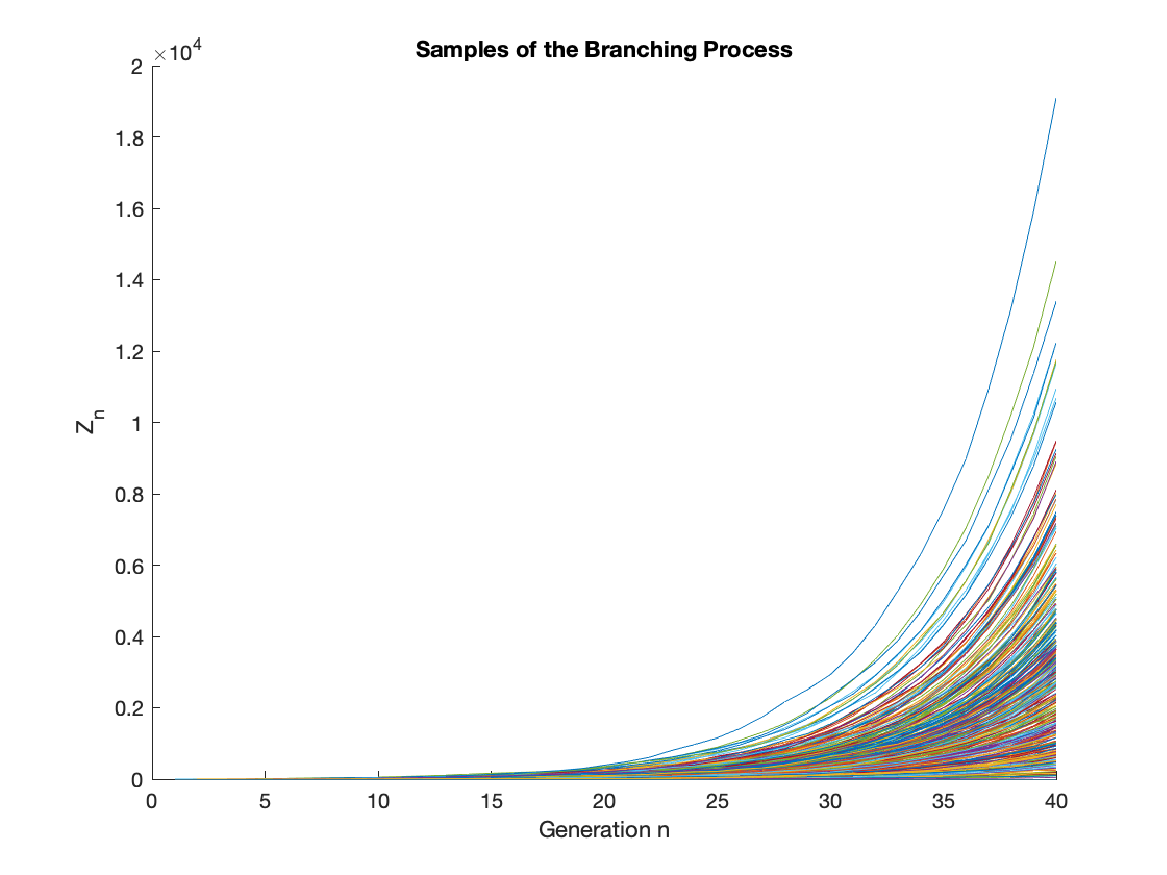
\includegraphics[scale=0.3]{img/0.png}}
                                \subfloat{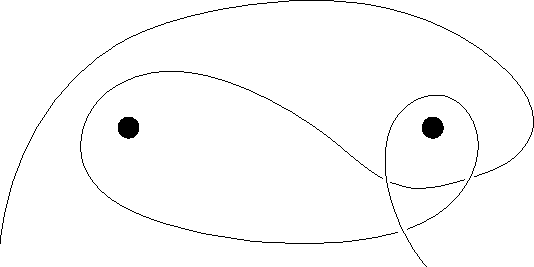
\includegraphics[scale=0.3]{img/1.png}}
				\subfloat{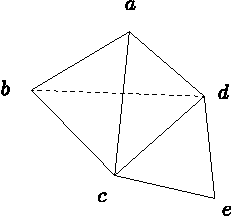
\includegraphics[scale=0.3]{img/2.png}}
                        \end{figure}

			Using the training data (500 random data points per class from a larget training set) and testing data (an additional 500 random data points per class from a larger testing set), multiple SVMs were trained with $C$ in $\{ 10^{-12}, 10^{-11}, \dots, 10^{12}\}$. The training and testing errors for each $C$ are plotted below.
			\begin{figure}[H]
                                \centering
				\subfloat{\includegraphics[scale=0.5]{img/mnist-acc.png}}
				\subfloat{\includegraphics[scale=0.5]{img/mnist-sv.png}}
                        \end{figure}
			From this we see that the testing accuracy is optimal (among the tested values of $C$) for $C=10^{-6}$. Is is around this value of $C$ that the algorithm seems to find the minimum number of support vectors, i.e. the maximum number of points have margin greater than 1.
	\end{enumerate}


%%%%%%%%%%%%%%%%%%%%
% AdaBoost
%%%%%%%%%%%%%%%%%%%%

\section{AdaBoost}

		\begin{enumerate}
			\item In lecture we showed that when the weak learning assumption holds, the error of AdaBoost decays exponentially, i.e.
			\[
				E_t = \frac{1}{n} \sum_{i=1}^{n} \mathbb{I}_{[y_i \neq H_t(y_i)]} \leq e^{-2t \gamma_{WLA}^2}.
			\] 
			Taking the limit as $t \to \infty$, we get $\lim_{t \to \infty} E_t \leq 0$. Since the error is non-negative, this implies that $\lim_{t \to \infty} E_t = 0$. Thus AdaBoost will correctly classify every point if the weak learning assumption holds.

		\item 
			Redefine $d_{t,i} = w_i e^{(-M \lambda_t)_i}/Z_t$. Now we must first find the descent direction $j_t$. The descent direction satisfies
		\[
			j_t = \arg\max_j \left[ -\frac{dR(\lambda_t + \alpha e_j)}{d \alpha} \Big|_{\alpha=0} \right].
		\] 
		Evaluating this derivative gives
		\begin{align*}
			-\frac{dR(\lambda_t + \alpha e_j)}{d \alpha} \Big|_{\alpha=0} &= -\frac{d}{d\alpha} \left( \sum_{i=1}^{n} w_i e^{[M(\lambda_t + \alpha e_j)]_i} \right)\Big|_{\alpha=0} \\
										      &= \sum_{i=1}^{n} \left( -\frac{d }{d \alpha} w_i e^{-(M \lambda_t)_i - \alpha M_{ij}} \right) \Big|_{\alpha=0} \\
										      &= \sum_{i=1}^{n} w_i M_{ij}e^{-(M \lambda_t)_i}
		\end{align*}
		The optimal $j$ for this expression will also maximize a normalized version of this sum, so we have
		\begin{align*}
			j_t &= \arg\max_j \left[ \left( \sum_{i=1}^{n} w_i M_{ij}e^{-(M \lambda_t)_i}\right) / Z_t \right] \\
			    &= \arg\max_j \sum_{i=1}^{n} M_{ij} d_{t,i} \\
			    &= \arg\max_j (d_t^T M)_j
		\end{align*}
		Note that this is the same expression as with standard AdaBoost, except with $d_ {t,i}$ defined differently. Now we must find the optimal distance to move in direction $j_t$.
		\begin{align*}
			0 &= \frac{dR(\lambda_t + \alpha e_j)}{d \alpha} \Big|_{\alpha=\alpha_t} \\
			0 &= \sum_{i=1}^{n} w_i M_{ij}e^{-(M\lambda_t)_i - \alpha_t M_{i{j_t}}} \\
			0 &= \sum_{i|M_{i{j_t}}=1} w_i e^{-(M\lambda_t)_i - \alpha_t} - \sum_{i|M_{i{j_t}}=-1} w_i e^{-(M\lambda_t)_i + \alpha_t} \\
			\intertext{Dividing both sides by $Z_t$ gives}
			0 &= e^{-\alpha_t} \Big[ \sum_{i|M_{i{j_t}}=1} d_{t,i} \Big] - e^{\alpha_t} \Big[ \sum_{i|M_{i{j_t}}=-1} d_{t,i} \Big] \\
			0 &= e^{-\alpha_t} (1-\varepsilon_t) - e^{\alpha_t} \varepsilon_t \\
			\alpha_t &= \frac{1}{2} \ln\left( \frac{1-\varepsilon_t}{\varepsilon_t}  \right)
		\end{align*}
		Note that this is also the same expression as with standard AdaBoost. Thus the only change to the algorithm is redefining $d_{t,i} = w_i e^{(-M \lambda_t)_i}/Z_t$. This only affects the initial weighting of the data points, not the weight updates, as
		\begin{align*}
			d_{t+1,i} &= w_i e^{-(M\lambda_{t+1})_i}/Z_{t+1}\\
				  &\propto w_i e^{-(M\lambda_t)_i} e^{-M_{i j_t} \alpha_t} \\
				  &\propto d_{t,i} \cdot e^{-M_{i j_t} \alpha_t}.
		\end{align*}
		This means that if we define $d_{1,i}$ based on the weights $w_i$, the rest of the algorithm will work unchanged.

		\begin{minipage}{\linewidth}
		\begin{algorithm}[H]
			Set $d_{1,i} = w_i$ for each $i$
			
			\For{$t=1$ to $T$}{
				Train weak classifier $h_t$ using the weak algorithm with data points weighted by $d_{t,i}$

				Choose coefficient $\alpha_t$ by
				\[
					\alpha_t = \frac{1}{2} \left( \frac{1-\varepsilon_t}{\varepsilon_t}  \right)
				\] 

				Update data weights by

				\uIf{$y_i = h_t(x_i)$ }{
					$d_{t+1,i} = d_{t,i} e^{-\alpha_t} / Z_t$
				} \Else{
					$d_{t+1,i} = d_{t,i} e^{\alpha_t} / Z_t$
				}
			}
			Output final classifier $H(x) = \text{sign}\left( \sum_{t=1}^{T} \alpha_t h_t(x) \right)$
			\caption{Weighted AdaBoost}
		\end{algorithm}
		\end{minipage}

		\item
			The stump weights for the constructed 10-stump ensemble are approximately
			\[
				\mathbf{w}=(0.17, 0.18, 0.10, 0.09, 0.07, 0.07, 0.06, 0.05, 0.03, 0.02).
			\] 
			These are not monotonically decreasing, but they \textit{almost} are. Since the decision stumps use only one feature, it appears that the most informative features (the ones selected first in the construction of the ensemble) are weighted most heavily. Thus the model gives these earlier features more weight when making a final decision.

			The training and testing accuracy for the dataset are plotted below vs. the number of iterations.

			\begin{figure}[H]
                                \centering
                                \includegraphics[scale=0.5]{img/boost-acc.png}
                        \end{figure}
			From this we see that there is not massive overfitting as the number of iterations increases. This is expected, as AdaBoost is known to be resistant to overfitting when using weak classifiers.

	\end{enumerate}
\end{document}
